\documentclass[border=10pt]{standalone}
\usepackage[svgnames]{xcolor}
\usepackage{amsmath}
\usepackage{pgfplots}
\pgfplotsset{compat=newest}
\usepackage[sfdefault]{FiraSans}
\usepackage{FiraMono}
\renewcommand*\familydefault{\sfdefault}
\begin{document}
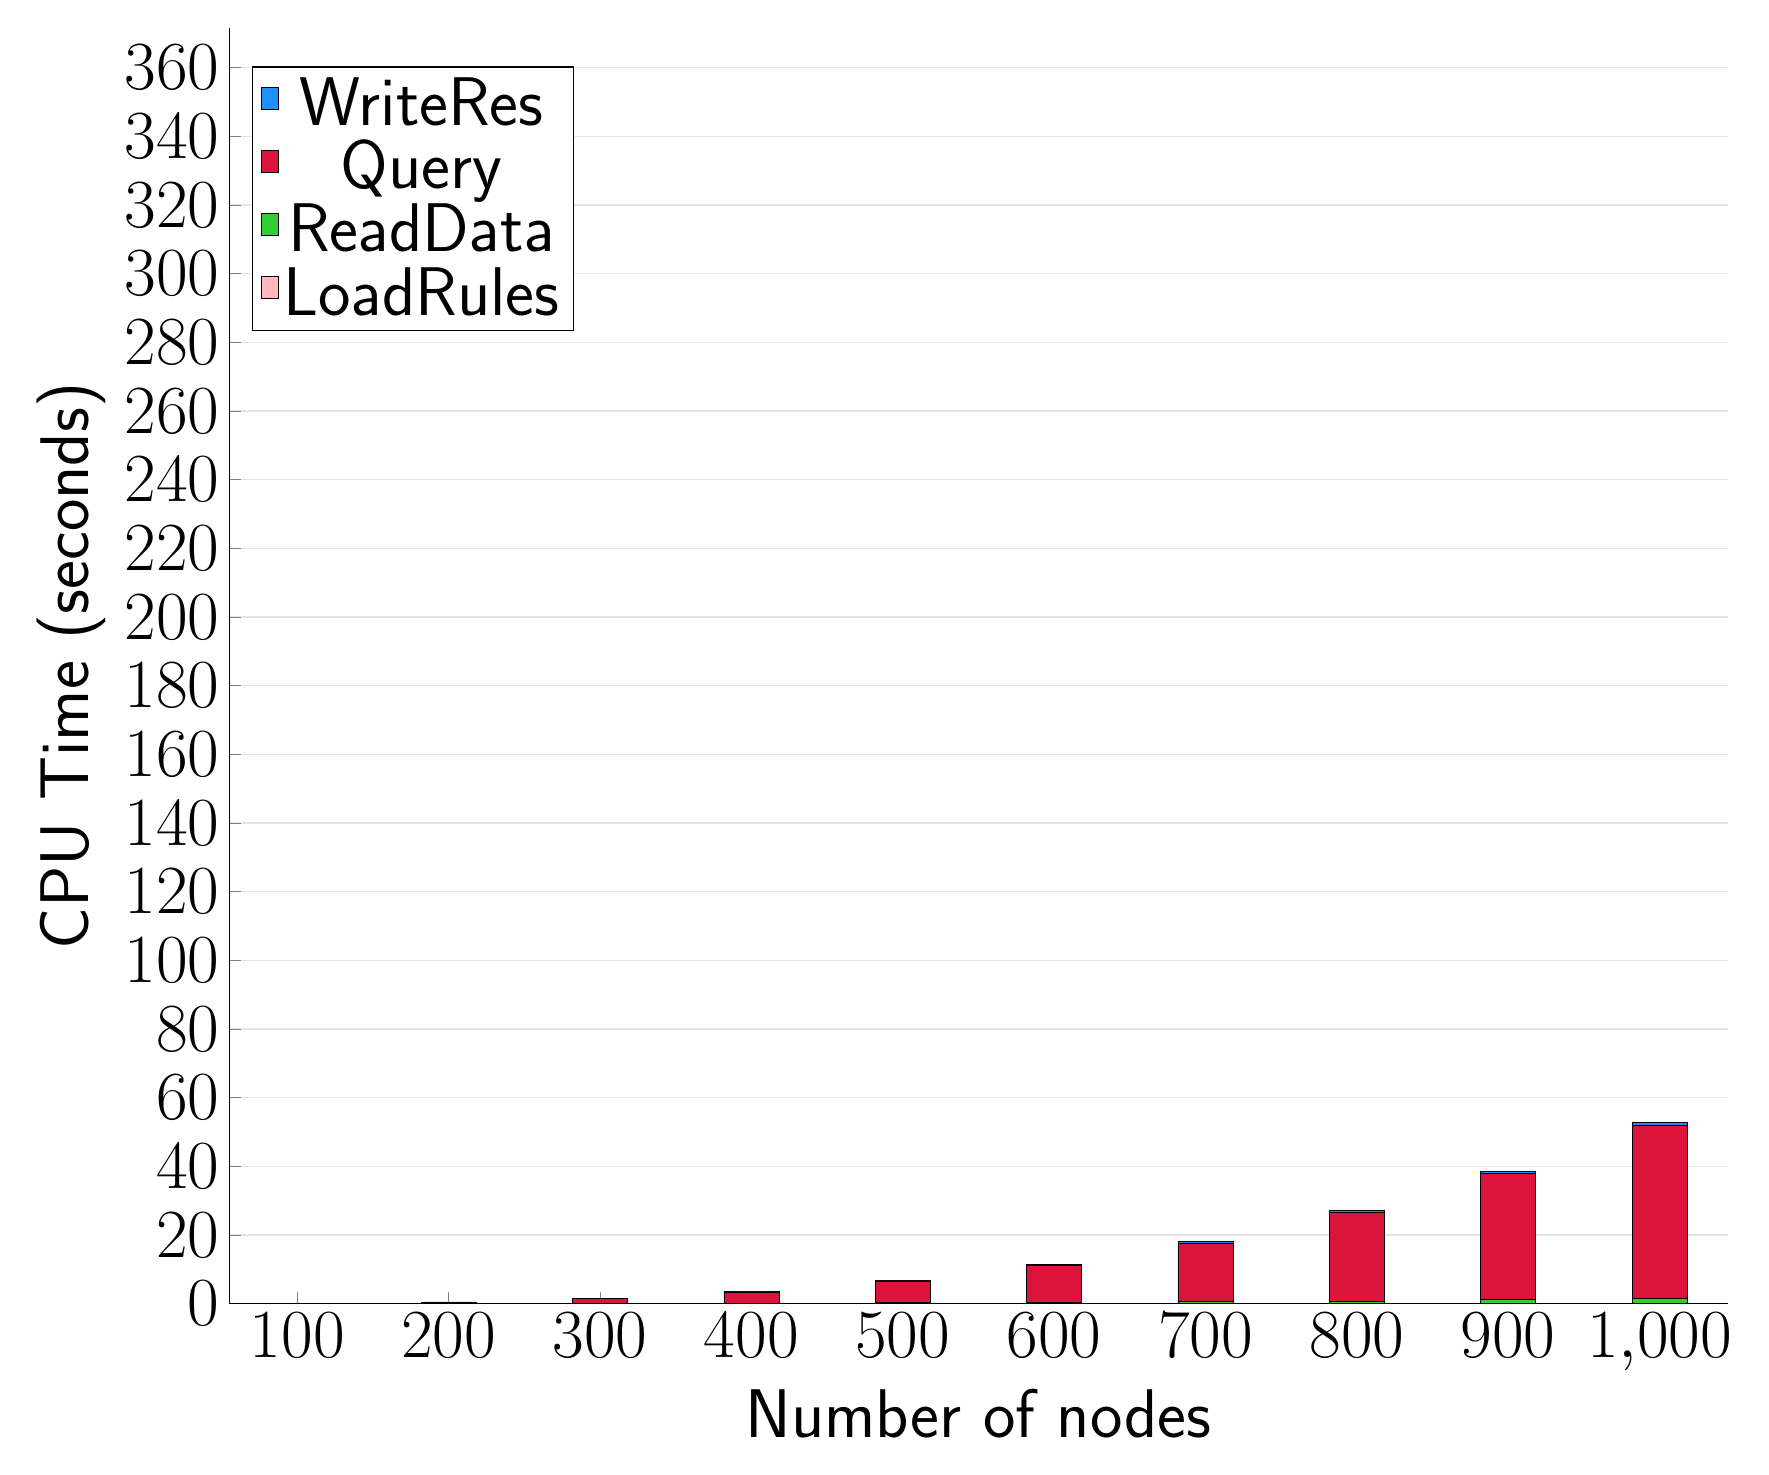
\begin{tikzpicture}
\begin{axis}[
   ybar stacked,
   width=1.7\textwidth,
   bar width=0.7cm,
   ymajorgrids, tick align=inside,
   major grid style={draw=gray!20},
   xtick=data,
   ymin=0, ymax=371.479,
   axis x line*=bottom,
   axis y line*=left,
   enlarge x limits=0.05,
   legend style={
       at={(0.23, 0.97)},
       anchor=north east,
       legend columns=1,
       font=\Huge,
   },
   ylabel={CPU Time (seconds)},
   xlabel={Number of nodes},
   label style={font=\Huge},
   tick label style={font=\Huge},
]
\addlegendimage{fill=DodgerBlue, draw=black, line width=0.2pt}
\addlegendentry{WriteRes}
\addlegendimage{fill=Crimson, draw=black, line width=0.2pt}
\addlegendentry{Query}
\addlegendimage{fill=LimeGreen, draw=black, line width=0.2pt}
\addlegendentry{ReadData}
\addlegendimage{fill=LightPink, draw=black, line width=0.2pt}
\addlegendentry{LoadRules}
\addplot +[fill=LightPink, draw=black, line width=0.2pt] coordinates {
(100, 0.0005237999999999999)
(200, 0.0005286000000000001)
(300, 0.0005498)
(400, 0.0005571999999999998)
(500, 0.000549)
(600, 0.0005493999999999994)
(700, 0.0005504)
(800, 0.0005488)
(900, 0.0005586000000000002)
(1000, 0.0005509999999999996)
};
\addplot +[fill=LimeGreen, draw=black, line width=0.2pt] coordinates {
(100, 0.0079604)
(200, 0.03473059999999999)
(300, 0.08631040000000001)
(400, 0.16369260000000002)
(500, 0.2691786)
(600, 0.41003179999999995)
(700, 0.5923489999999999)
(800, 0.8272485999999999)
(900, 1.1285733999999998)
(1000, 1.4986244)
};
\addplot +[fill=Crimson, draw=black, line width=0.2pt] coordinates {
(100, 0.0512988)
(200, 0.41823460000000007)
(300, 1.3828673999999999)
(400, 3.2612724)
(500, 6.3743162)
(600, 10.784925999999999)
(700, 17.092316)
(800, 25.7518712)
(900, 36.7854144)
(1000, 50.5288714)
};
\addplot +[fill=DodgerBlue, draw=black, line width=0.2pt] coordinates {
(100, 0.0088542)
(200, 0.0318306)
(300, 0.07129500000000007)
(400, 0.13178220000000004)
(500, 0.21979000000000007)
(600, 0.2560396000000001)
(700, 0.3964343999999997)
(800, 0.5250039999999998)
(900, 0.5587401999999997)
(1000, 0.6592963999999994)
};
\end{axis}
\end{tikzpicture}

\end{document}
